\begin{figure}[t]
\centering

\includegraphics[width=\columnwidth]{sidekick-paper/figures/fig5_baseline_bar_legend.pdf}
\begin{subfigure}{0.49\linewidth}
	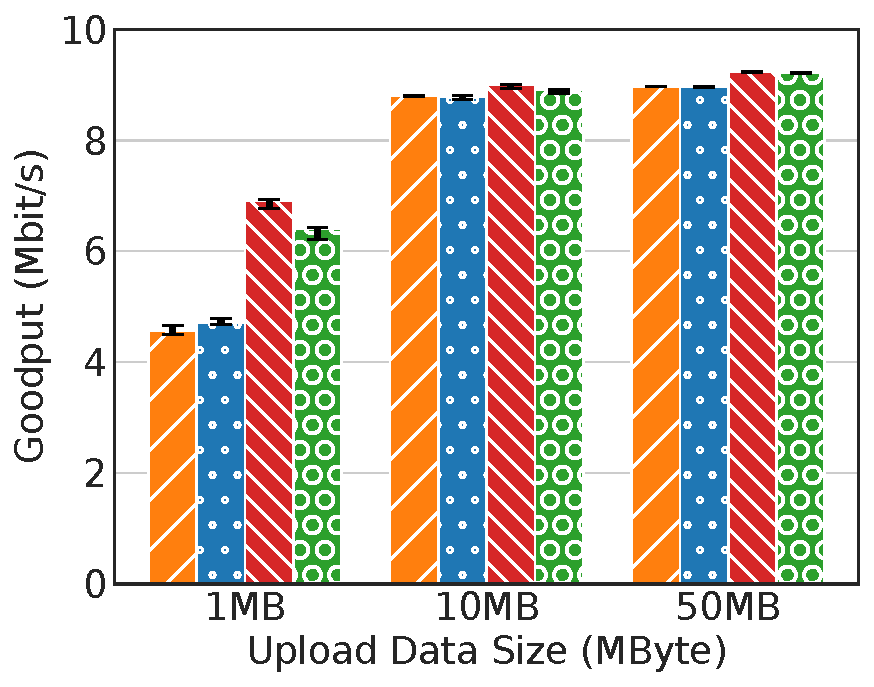
\includegraphics[width=\linewidth]{sidekick-paper/figures/fig5_baseline_loss0p.pdf}
	\caption{0\% loss.}
	\label{fig:baseline-bar:loss0p}
\end{subfigure}
\begin{subfigure}{0.49\linewidth}
	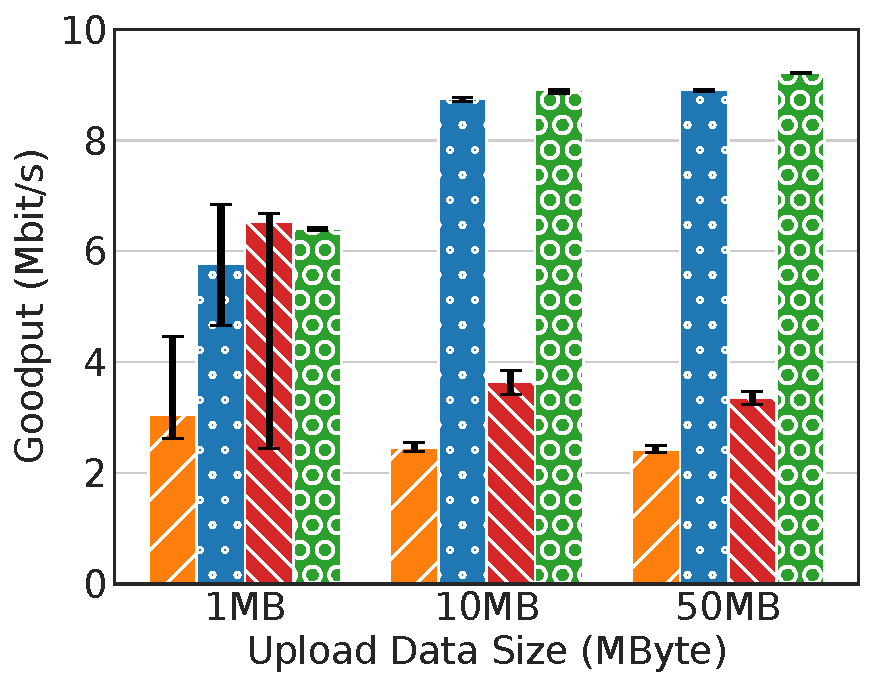
\includegraphics[width=\linewidth]{sidekick-paper/figures/fig5_baseline_loss1p.pdf}
	\caption{1\% loss.}
	\label{fig:baseline-bar:loss1p}
\end{subfigure}
\caption{Median goodput for three upload data sizes with $0\%$ and $1\%$ loss on
Link 1. 20 trials. Error bars are 1st and 3rd quartiles.
With proxy assistance at $1\%$
loss, both QUIC and TCP match the performance of when there is no loss at all.
}
\label{fig:baseline-bar}
\end{figure}

\begin{figure}[t]
\centering

\includegraphics[width=\columnwidth]{sidekick-paper/figures/fig6_legend.pdf}
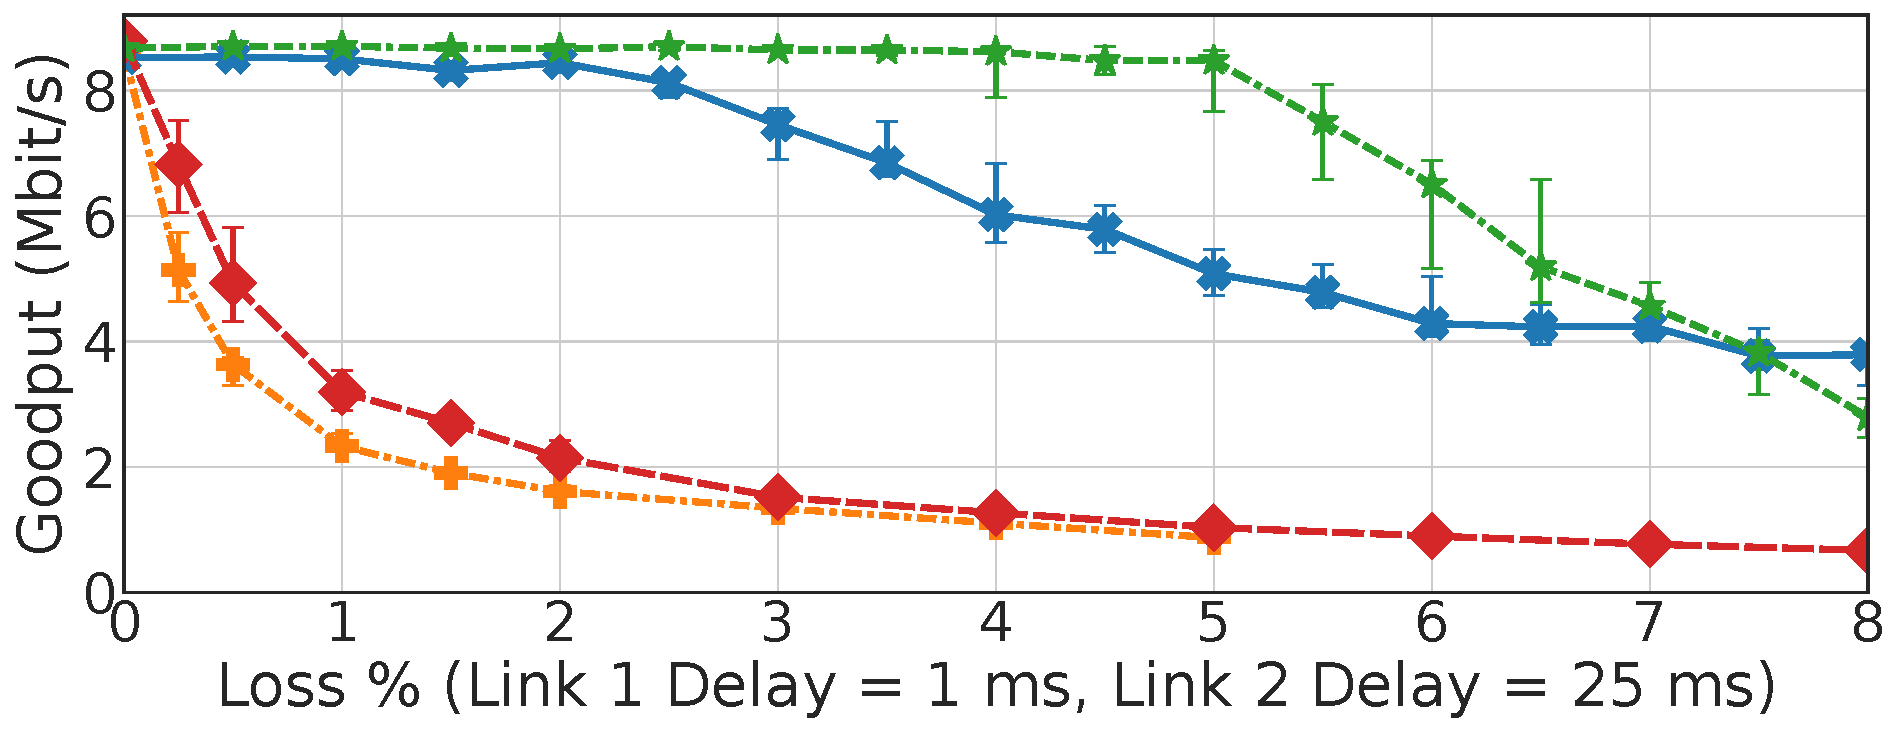
\includegraphics[width=\columnwidth]{sidekick-paper/figures/fig6_loss_bw100_10M_delay_25ms_1ms.pdf}
\caption{Connection-splitting PEP emulation as a function of near-segment
	loss rate. In this emulation experiment, QUIC+Sidekick (running PACUBIC)
  performs similarly to TCP+PEP (each connection running CUBIC)
  and improves goodput compared with end-to-end protocols. The graph shows
  median goodput of a 10~MByte upload. QuACK interval is 30~ms, threshold
is 10. Error bars show IQR of 10 trials.
}
\label{fig:loss-vs-tput}
\end{figure}
